\begin{document}
\graphicspath{ {images/slt/} }

\section{Structure Learning -- Trees}

\subsection{Structure Learning for an Undirected Tree-Structured Graphical Model: The Chow-Liu Algorithm}

At this point we've covered parameter learning for undirected trees, where we assume we know the tree structure. But what if we don't know what tree to even use? We now look at an algorithm called the Chow-Liu algorithm that learns which tree to use from training data, again using maximum likelihood. Once more, information measures appear, where mutual information plays a pivotal role. Recall that mutual information tells us how far two random variables are from being independent. A key idea here is that to determine whether an edge between two random variables should be present in a graphical model, we can look at mutual information.

The idea is that we have random variables $X_1$ up through $X_k$. These you can think of as nodes in a undirected graphical model. But we don't know which edges should be in this graphical model. And restricting ourself to trees, the question is, which tree should we use? To help us answer this question, we're going to have access to training data. We see $n$ i.i.d. samples from this graphical model, where for each of the samples, of course, we see everything, $x_1^{(i)},\dots ,x_k^{(i)}$. So this is the $i$-th training data point and $i = 1 \dots n$. Just as a comment, the number of possible trees here is humongous, actually $k^{k-2}$. This from a result called Cayley's formula, which grows even faster than exponential, it's super exponential. Somehow, we're going to search this huge space of possible trees to select the best tree. It turns out, doing that can be done very quickly. To select the tree we're going to use maximum likelihood. We're going to pick the tree $T$ here. 

{\centering$\displaystyle \widehat{T}=\arg\max_{T} \bigg\{\max_{\theta_T} \log \prod_{i=1}^n p_{x_1 \dots x_k} (x_1^{(i)},\dots ,x_k^{(i)}; T, \theta_T) \bigg\}$ \par}

In this case, we know that there are $k$ nodes, but where are the edges? You can think of $T$ as just specifying which edges are present that result in a tree across $k$ nodes, with $k-1$ edges. So we're trying to find the best tree such that once we fix a tree, then we can do maximum likelihood for that specific tree $T$. 

To solve this optimization problem, it turns out there's a very clean algorithm. To get to it, we're going to simplify what's in the curly braces:

\begin{eqnarray*}
\text{For specific tree } T: \\
& & \max_{\theta_T} \log \prod_{i=1}^n p_{x_1 \dots x_k} (x_1^{(i)},\dots ,x_k^{(i)}; T, \theta_T)  \\&=& \log \prod_{i=1}^n \bigg[ \widehat{p}(x_r^{(i)}) \prod_{j \ne r} \widehat{p}(x_r^{(i)} | x_{\pi(j)}^{(i)}) \bigg] \\
&=& \sum_{i=1}^n \log \widehat{p}(x_r^{(i)}) + \sum_{j \ne r} \sum_{i=1}^n \log \widehat{p}(x_r^{(i)} | x_{\pi(j)}^{(i)}) \\
\end{eqnarray*}

We have the log likelihood across the training data. Here, we're parameterizing by both what the tree is and then, once we know the tree, some set of parameters $\theta_T$ for the tree. We can arbitrarily choose a root $r$ and drop the subscripts just to save some writing. So the factorization is $p(x_r^{(i)})$ times the product from all the nodes that are not equal to the root $p(x_r^{(i)} | x_{\pi(j)}^{(i)})$. We want to take the maximum over all the $\theta_T$'s, meaning we want to plug in the best possible values of the parameters into this expression. But we know from the parameter learning video that the best choice of $\theta$ is going to correspond to the empirical distributions. All we need to do is replace the probability distributions $p$ with the empirical versions $\widehat{p}$, which give us the desired max. As a reminder, $\widehat{p}(x_r^{(i)})$ is the empirical distribution of random variable $X_r$. Evaluated at some value $a$ this is just equal to the fraction of times $a$ appears in the training data. So $\widehat{p}(x_r^{(i)}) = \frac{1}{n} \sum_{i=1}^n \mathbf{1} \{x_r^{(i)}=a\}$. This is just an example of how you get these empirical distributions. The empirical conditional probability table, as a reminder, is going to be the fraction of times we see that these two random variables in our training data jointly take on two specific values divided by the number of times we see this random variable taking on a specific value in our training data. That's what these $\widehat{p}$'s are. 

\begin{eqnarray*}
& & \sum_{i=1}^n \log \widehat{p}(x_r^{(i)}) + \sum_{j \ne r} \sum_{i=1}^n \log \widehat{p}(x_r^{(i)} | x_{\pi(j)}^{(i)}) \\
&=& \sum_a \bigg[ \sum_{i=1}^n \mathbf{1} \{ x_r^{(i)} = a\} \bigg] \log \widehat{p}_{x_r} (a) + \sum_{j \ne r} \sum_{a,b} \bigg[ \sum_{i=1}^n \mathbf{1} \{ x_j^{(i)} = a, x_{\pi(j)}^{(i)} = b \} \bigg] \log \widehat{p}_{x_j | x_{\pi(j)}} (a|b) 
\end{eqnarray*}

Next we introduce a different summation to split up what the possible values of this random variable are. We were doing this for the conditional distributions earlier. But now, we're going to do it for all of them, counting up how many times we see each particular value. %You can use the definition of conditional probability even for an empirical distribution, because an empirical distribution is still a distribution. So we can write this piece as p hat of X j, X pi j of a comma b divided by-- and then since we're conditioning on X pi j, it's going to be p hat of X pi j evaluated at b. So we're going to have this. A

\begin{eqnarray*}
& & \sum_a \underbrace{\bigg[ \sum_{i=1}^n \mathbf{1} \{ x_r^{(i)} = a\} \bigg] \log \widehat{p}_{x_r} (a)}_{n p_{x_r} (a)} + \sum_{j \ne r} \sum_{a,b} \underbrace{\bigg[ \sum_{i=1}^n \mathbf{1} \{ x_j^{(i)} = a, x_{\pi(j)}^{(i)} = b \} \bigg]}_{n \widehat{p}_{x_j, x_{\pi(j)}} (a,b) } \log \widehat{p}_{x_j | x_{\pi(j)}} (a|b) \\
&=& n \bigg[ \underbrace{\sum_a p_{x_r} (a) \log \widehat{p}_{x_r} (a)}_{-H(\widehat{p}_{x_r})} + \underbrace{\sum_{j \ne r} \sum_{a,b} \widehat{p}_{x_j, x_{\pi(j)}} (a,b) \log \frac{ \widehat{p}_{x_j, x_{\pi(j)}} (a,b) }{ \widehat{p}_{x_{\pi(j)}} (b) \widehat{p}_{x_j}(a)} }_{\sum_{j \ne r} D(\widehat{p}_{x_j, x_{\pi(j)}})} \widehat{p}_{x_j}(a) \bigg] \\
&=& n \bigg[ -H(\widehat{p}_{x_r}) + \sum_{j \ne r} \underbrace{D(\widehat{p}_{x_j, x_{\pi(j)}})}_{\widehat{I}(x_j, x_{\pi(j))}} + \underbrace{\sum_a \widehat{p}_{x_j}(a) \log \widehat{p}_{x_j}(a)}_{-H(\widehat{p}_{x_j}} \bigg] \\
&=& n \bigg[ -\sum_{j \in V} H(\widehat{p}_{x_j}) + \sum_{(i,j) \in E} \widehat{I}(x_i;x_j) \bigg]
\end{eqnarray*}

The first term is related to the negative entropy. The log is natural log, but that's OK. We can still talk about the entropy, it's just in terms of ``nats'' not bits. The second term we multiply top and bottom by $\widehat{p}_{x_j}(a)$, which is just multiplying by 1. That gives us a term which is the information divergence $D(\widehat{p}_{x_j, x_{\pi(j)}})$. The basic idea is we're looking at how far the empirical joint distribution is from a product of two empirical marginal distributions. You can think of this as saying, how far is this empirical joint distribution from being independent. This is called the mutual information between these two random variables. But it's not actually these two random variables, it's the empirical versions of them. So we'll denote this as the empirical mutual information between $x_j$ and $x_{\pi(j))}$. Again, the mutual information would be this exact same thing except with the true distributions, rather than the empirical distributions. Now, when we're looking at the empirical distributions, we just get this empirical mutual information instead. So that accounts for one piece of the second term. We have another piece, and this will become a minus entropy of the empirical distribution of $X_j$. Once we put all these pieces together, there is a minus entropy of the root node and a minus entropy for all the other nodes. So we're going to have a sum over all the nodes $V$ of minus entropy of the empirical distribution of $X_j$. We're also going to have the empirical mutual information $\widehat{I}(x_i;x_j)$ for $(i, j)$ within the edges in the tree.

The bottom line is this is equal to the maximum likelihood across parameters for a specific tree $T$. Note that to choose the best possible tree, the nodes aren't going to change, so the negative entropy term is going to be the same across any tree. The only thing that changes is the mutual information term that depends on the edges in the tree. So to figure out what the best tree is possible we just want to maximize this $\sum_{(i,j) \in E} \widehat{I}(x_i;x_j)$ term. 

Now we want an algorithm that maximizes this across all possible trees. The basic idea of the algorithm is to start with a graph with no edges and incrementally add edges until we get the best tree according to maximum likelihood. For the first edge we add, we're going to look at all pairs of random variables to find which one has the highest empirical mutual information, and we're going to add that edge. Then we're going to repeat that process -- we're going to find the pair of random variables with the second-highest empirical mutual information and so forth where we make sure that whenever we add an edge we don't introduce a cycle. And after we add enough edges we're going to get a tree and that's actually the best tree. This is called the Chow-Liu algorithm, illustrated with a simple four-node example. 

{\centering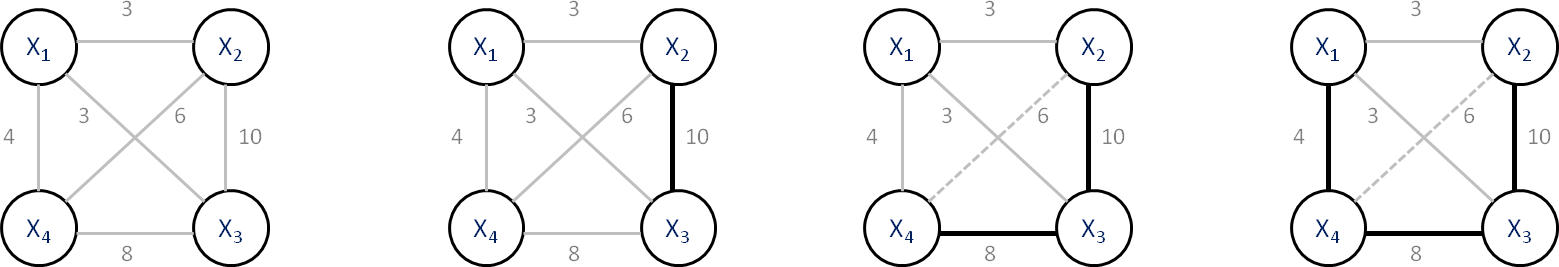
\includegraphics[scale=0.4]{Chow_Liu4a} \par}

Here we have $k=4$ for $X_1 \dots X_4$, and in gray are all the edges you could possibly have. For each of these edges we have a gray number, the empirical mutual information quantities. In practice these would be computed based on your training data. In the Chow-Liu algorithm we ask, what is the highest empirical mutual information? It's 10, so that is first edge to be added. The second highest edge is 8, which we add. Then in the next step, the third highest one is 6, but if we add this edge it will form a cycle, so skip that and move on to the next highest, which is 4, and we add that. At this point the algorithm would stop because adding anything else would form a cycle. So at this point the Chow-Liu algorithm would output a tree, denoted by the solid black lines, and that would be the maximum likelihood estimate for the best possible tree we could use. 

The general idea is very simple. We start with a graph with no edges. And then for all pairs of random variables $(i,j)$ we compute the empirical mutual information quantities $\widehat{I}(X_i; X_j)$, the gray numbers. Next we sort these empirical mutual information quantities from highest to lowest. And then starting from the highest and going all the way to the lowest we're going to add edges, except we skip adding an edge if it results in a cycle. And this algorithm will always terminate because for a graph with $k$ nodes, any tree for that graph is going to have $k-1$ edges. For example in this case, any tree for this graph has 3 edges. That is the Chow-Liu algorithm. Given training data we can learn what is the maximum likelihood estimate for the tree that best explains the data. 


\subsection{Correctness and Running Time of the Chow-Liu Algorithm}

These notes fill in details for why the Chow-Liu algorithm is correct and what its running time is. As a reminder, these notes are inherently more advanced and meant for those who are interested in the gory details.

We already justified why the maximum likelihood tree is the solution to the optimization problem

{\centering$\widehat{T}=\arg \max _{T\text { that is a tree over nodes }\{ 1,\dots ,k\} }\sum _{(i,j)\in T}\widehat{I}(X_{i};X_{j}).$ \par}
 
Here, we treat $T$ as a set of edges, where edge $(i,j)$ is the same as edge $(j,i)$ so for simplicity we ask that $i<j$. As illustrated in the video, we can think of the above optimization problem as the following:

\begin{enumerate}
\item For every pair of nodes $i$ and $j$ with $i<j$, there is a possible edge $(i,j)$ that can belong to the best tree $\widehat{T}$. If edge $(i,j)$ is in $\widehat{T}$, then it contributes a ``reward'' of $\widehat{I}(X_{i};X_{j})$ to the sum that we are maximizing over.

\item Thus, the question is: What is the tree composed of edges that have the highest overall reward?
\end{enumerate}

It turns out that this problem has been widely studied in computer science and amounts to finding what is called the ``minimum weight spanning tree'' (often shortened to just minimum spanning tree or MST). Note that we can easily turn the problem into one of getting the tree with the minimum overall weight (instead of maximum overall empirical mutual information) by associating the weight $w\big ((i,j)\big )\triangleq -\widehat{I}(X_{i};X_{j})$ for each edge $(i,j)$, and then solving the equivalent optimization problem

{\centering$\widehat{T}=\arg \min _{T\text { that is a tree over nodes }\{ 1,\dots ,k\} }\sum _{(i,j)\in T}w\big ((i,j)\big ).$ \par}
 
The solution $\widehat{T}$ is called a minimum weight spanning tree because it is a tree that reaches (and thus ``spans'') all the possible nodes (so from any node, we can reach any other node by traversing edges along the tree), and if we sum up the weights associated with all the edges in the tree, we get the minimum possible overall weight.

Thus, the correctness of the Chow-Liu algorithm hinges on the correctness of established algorithms for solving the MST problem. One of the most popular algorithms for solving the MST problem is Kruskal's algorithm, which is what we covered in the Chow-Liu video:

\begin{itemize}
\item Start with no edges and repeatedly add the next lowest weight edge that doesn't introduce a cycle. (Again, lower weight means higher empirical mutual information here.)
\end{itemize}

What remains is to show why the Chow-Liu algorithm is correct (which given our analysis thus far amounts to just showing why Kruskal's algorithm is correct) and how long it takes to run. After all, anyone can write an algorithm that produces a wrong answer in $\mathcal{O}(1)$ time, and moreover, even if the algorithm is correct, if it has to loop through all $K^{k-2}$ possible trees, then the algorithm would be practically useless for large values of $k$!

\textbf{Bibliographic note.} In what follows, we are largely following the exposition of Kruskal's algorithm in Dasgupta, Papadimitriou, and Vazirani's textbook ``Algorithms'' McGraw-Hill 2006 (Section 5.1).

\subsection{Correctness of Kruskal's Algorithm}

As we have already established previously in the course, a tree on $k$ nodes has exactly $k-1$ edges. The intuition for the proof of this is that starting from a fully disconnected graph, by adding edges, every time we are merging exactly two connected components (a connected component is a collection of nodes that are all reachable from each other and that has no edges to any other nodes outside of the connected component). By starting with $k$ connected components, after merging two connected components exactly $k-1$ times, we are left with a single connected component, and adding any other edge would result in a cycle (since all the nodes are already in the same connected component). Note that this way in which a tree is built up is precisely how Kruskal's algorithm builds up a tree: each time an edge is added, exactly two different connected components are merged (it cannot be that the edge added is between two nodes in the same connected component since that would mean that adding it would produce a cycle as the nodes are already connected via some other path). After $k-1$ edges are added, all the nodes are in the same connected component, meaning that the edges added so far correspond to a graph that is connected (i.e., any node can reach any other node by traversing edges in the graph) and that also covers every node.

In fact, a key property of trees is that any graph over $k$ nodes that is both connected and has $k-1$ edges must be a tree. The reason why this is true is to note that if we take a graph over $k$ nodes that is connected and has $k-1$ edges, then if there were cycles, we could remove any cycles to end up with a tree that is still connected over the $k$ nodes. However, we know that any tree over $k$ nodes has $k-1$ edges, so it must mean that we didn't remove any edges, i.e., the graph was indeed a tree to begin with. So we know that the resulting graph built by Kruskal's algorithm is a tree that spans all $k$ nodes.

The main technical challenge is justifying that the spanning tree produced by Kruskal's algorithm is of minimum weight. To show this, the high level idea is to show that every time Kruskal's algorithm adds an edge, the resulting graph (which is not yet a tree until we add $k-1$ edges) is a subset of a possible MST. (Note: In general, there could be multiple MST's for the same set of nodes and choice of weights on the possible edges.) Thus, after adding $k-1$ edges, the resulting graph is still part of an MST over $k$ nodes, but this means that the graph at this point must itself be an MST since the graph is already a spanning tree over $k$ nodes.

To show this result, we do a graph induction. Let $E_{\ell }$ be the set of the first $\ell$ edges added by Kruskal's algorithm. We aim to prove the proposition that for each $\ell =0,1,\dots ,k-1$, there exists an MST (represented as a set of edges) that contains $E_{\ell }$ as a subset of edges.

Base case $(\ell=0)$: At this point $E_0 =\emptyset$, and clearly any MST has the empty set as a subset of the edges.

Inductive step: Suppose the proposition above holds for $\ell =m$ for $0\le m<k-1$. We want to show that it also holds for $\ell=m+1$. Let $T^{*}$ be the MST that contains $E_m$. Let $e$ be the edge that Kruskal's algorithm adds, so that $E_{m+1}=E_{m}\cup \{ e\}$. There are two cases to consider.

\begin{itemize}
\item If $E_{m+1}\subseteq T^{*}$, then we're done: $E_{m+1}$ is also contained within an MST, namely $T^{*}$.

\item If instead $E_{m+1}\not\subseteq T^{*}$, then now we need to show that $E_{m+1}$ is instead contained in a different MST. Since $E_{m}\subseteq T^{*}$, then it must be that the edge added $e$ is not in $T^{*}$. Thus, $T^{*}\cup \{ e\}$ contains a cycle $C$ which involves the edge $e$. This cycle $C$ must contain another edge $e'$ that is not in $E_m$. (Otherwise, it means that all the other edges in $C\setminus \{ e\}$ are in $E_m$ in which case Kruskal's algorithm could not have added edge $e$ as it would have created the cycle $C$ in producing $E_{m+1}$.) Then consider the set of edges $T^{\dagger }\triangleq T^{*}\cup \{ e\} \setminus \{ e'\}$, i.e., we take the MST $T^{*}$ that contained $E_m$, add edge $e$, and remove edge $e'$. Note that

{\centering$E_{m+1}\subseteq T^{\dagger }.$ \par}

\end{itemize}
 
This holds since $E_{m}\subseteq T^{*}$, edge $e'$ is neither in $E_m$ nor $E_{m+1}$, and we added edge $e$ to get from Em to $E_{m+1}$.

The final claim here is that the set of edges $T^{\dagger }$ actually corresponds to an MST. First off, note that $T^{\dagger }$ is connected and spans all the nodes. The reason why this is the case: We produce $T^{\dagger }$ by taking the MST $T^{*}$, adding edge $e$ (which produces cycle $C$), and then removing edge $e'$ (which is in cycle $C$). Note that for any graph that has a cycle, removing an edge from that cycle cannot disconnect the graph. In particular, all $k$ of the nodes remain connected in $T^{\dagger }$ (i.e., there is a path to reach from any node to any other node), and there are $k-1$ edges, so $T^{\dagger }$ is again a tree that spans all $k$ nodes.

As to why $T^{\dagger }$ has minimum weight, the key observation is that edges $e$ and $e'$ are both edges that are not in $E_m$, and so since Kruskal's algorithm added edge $e$ to go from $E_m$ to $E_{m+1}$, it must be that the weight $w(e')$ associated with $e'$ is at least equal to the weight $w(e)$ of $e$. (If $w(e')$ had actually been less than $w(e)$, then since $E_{m}\subseteq T^{*}$ and $e'\in T^{*}$, then Kruskal's algorithm would have added edge $e'$ instead since it certainly wouldn't have introduced a cycle.) We conclude that

{\centering$\text {weight of }T^{\dagger }=\text {weight of }T^{*}-\underbrace{w(e')}_{\ge w(e)}+w(e)\le \text {weight of }T^{*},$ \par}
 
so the weight of $T^{\dagger }$ is upper-bounded by the weight of $T^{*}$. But since $T^{*}$ is an MST, then it must be that the weight of $T^{\dagger }$ cannot actually be lower so it too is an MST.

This completes the proof of the inductive step for why the edges $E_{m+1}$ are also contained in an MST.

We thus conclude that for each $\ell =0,1,\dots ,k-1$, the intermediate edge set $E_{\ell }$ is contained in an MST. Then since $E_{k-1}$ corresponds to a connected graph over nodes $\{1,\dots,k\}$ with $k-1$ edges, it is a spanning tree, and as it is contained in an MST, it must itself be an MST since an MST over a graph of $k$ nodes has exactly $k-1$ edges.

\subsection{Running Time of the Chow-Liu Algorithm}

The running time of Chow-Liu is the running time of computing all the empirical mutual information quantities followed by the running time of Kruskal's algorithm, where the tricky part in analyzing the running time of Kruskal's algorithm is looking at how long it takes to detect cycles.

\textbf{Running time of computing empirical mutual information quantities.} Let's first look at the time complexity of computing $\widehat{I}(X_{i};X_{j})$ for all $i<j$. We compute the empirical marginal distributions

{\centering$\widehat{p}_{X_{i}}(a)=\frac{1}{n}\sum _{\ell =1}^{n}\mathbf{1}\{ x_{i}^{(\ell )}=a\} ,$ \par}
 
for every $i\in \{ 1,\dots ,k\}$ and every item in the alphabet; let's suppose that the alphabet size for all the $X_i$'s is $|\mathcal{X}|$. Then the running time to do this is $\mathcal{O}(k|\mathcal{X}|n)$.

Next we compute all the empirical pairwise distributions

{\centering$\widehat{p}_{X_{i},X_{j}}(a,b)=\frac{1}{n}\sum _{\ell =1}^{n}\mathbf{1}\{ x_{i}^{(\ell )}=a,x_{j}^{(\ell )}=b\}$ \par}
 
for every $i<j$ and every pair of items in the alphabets. The running time to do this is $\mathcal{O}(k^{2}|\mathcal{X}|^{2}n)$, where we recall that there are ${k \choose 2}=\mathcal{O}(k^{2})$ possible pairs.

Finally, we compute all ${k \choose 2}$ empirical mutual information quantities

{\centering$\widehat{I}(X_{i};X_{j})=\sum _{a}\sum _{b}\widehat{p}_{X_{i},X_{j}}(a,b)\log \frac{\widehat{p}_{X_{i},X_{j}}(a,b)}{\widehat{p}_{X_{i}}(a)\widehat{p}_{X_{j}}(b)}.$ \par}
 
Given that we have already computed the empirical distributions, this takes time $\mathcal{O}(k^{2}|\mathcal{X}|^{2})$.

Thus, all together, computing the empirical distributions and the empirical mutual information quantities takes a total of $\mathcal{O}(k^{2}|\mathcal{X}|^{2}n)$ operations (the complexity is dominated by computing the empirical pairwise distributions).

\textbf{Running time of Kruskal's algorithm.} Let's be clear about what the algorithm's steps are. We will use something called a Union-Find data structure to help us prevent cycles from being added. This data structure has three parts to it:

\begin{itemize}
\item To initialize the Union-Find data structure, every node is set to be its own connected component in the graph. Initializing every node to be its own connected component corresponds to when all the nodes are disconnected. This initialization takes time $\mathcal{O}(k)$.

\item Given a node $i$, there is a function $find(i)$ that finds which connected component $i$ belongs to. Each call to find takes time $\mathcal{O}(\log k)$.

\item Given two nodes $i$ and $j$, there is a function $union(i,j)$ that merges the connected components of $i$ and $j$ into a single connected component. Each call to union takes time $\mathcal{O}(\log k)$.
\end{itemize}

Details on the Union-Find data structure are given later.

We can now state Kruskal's algorithm as follows:

\begin{enumerate}
\item Set the edges added to the tree so far to be $T=\emptyset$. (Takes $\mathcal{O}(1)$ time.)

\item Initialize the Union-Find data structure, setting every node to be its own connected component. (Takes $\mathcal{O}(k)$ time.)

\item Sort all the possible edges (i.e., all ${k \choose 2}$ pairs) by their weights. (Using quicksort or mergesort, this takes $\mathcal{O}(k^{2}\log k^{2})=\mathcal{O}(2k^{2}\log k)=\mathcal{O}(k^{2}\log k)$ time.)

\item For each pair of nodes $(i,j)$ with $i<j$ and in increasing order of weight: (Worst case: ${k \choose 2}$ total iterations)

\begin{itemize}
\item If $find(i)\ne find(j)$, meaning that $i$ and $j$ are in different connected components: (this check takes $\mathcal{O}(\log k)$ time)

\begin{enumerate}
\item Set $T=T\cup \{ (i,j)\}$. (Takes $\mathcal{O}(1)$ time.)

\item Call $union(i,j)$ to merge the connected components of $i$ and $j$. (Takes $\mathcal{O}(\log k)$ time.)
\end{enumerate}
\end{itemize}
\end{enumerate}

Thus, putting together the pieces, the worst-case running time for Kruskal's algorithm is

{\centering$\underbrace{\mathcal{O}(1)+\mathcal{O}(k)}_{\text {initialization}} +\underbrace{\mathcal{O}(k^{2}\log k)}_{\text {sorting}} +\underbrace{{k \choose 2}\big (\mathcal{O}(\log k)+\mathcal{O}(1)+\mathcal{O}(\log k)\big )}_{\text {adding edges}}=\mathcal{O}(k^{2}\log k).$ \par}
 
Recall that computing all the empirical mutual information quantities takes time $\mathcal{O}(k^{2}|\mathcal{X}|^{2}n)$, where $|\mathcal{X}|$ is the alphabet size of each variable (or you can treat this as the maximum alphabet size of any variable), and $n$ is the number of training data. Thus, the overall time complexity of the Chow-Liu algorithm is

{\centering$\mathcal{O}(k^{2}|\mathcal{X}|^{2}n+k^{2}\log k).$ \par}
 
This running time is certainly a massive improvement over trying to iterate through all $k^{k-2}$ possible trees!

\subsection{Details on the Union-Find Data Structure}

We first sketch out with an example how the Union-Find data structure works. The basic idea of the Union-Find data structure is to represent all the connected components in a \textit{directed} graph over the $k$ nodes. A directed graph, unlike an undirected graph, has orientation associated with each edge. A connected component is encoded as all nodes where if you keep following the arrows, you reach the same node that is its own parent. We'll illustrate what this means shortly.

Initialization involves setting each node to be its own parent:

{\centering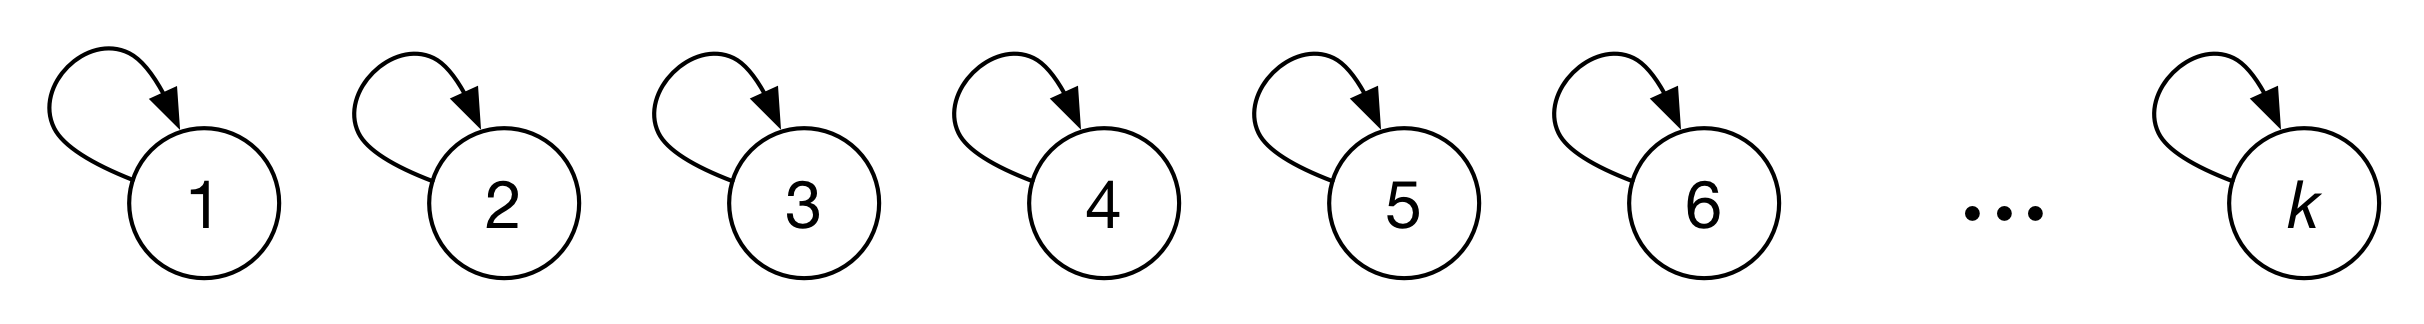
\includegraphics[scale=0.4]{images_union-find1} \par}

Here, notice that since each node is its own parent, it means that there are $k$ different connected components.

Next, consider what happens when we add an edge, say $(1,2)$. This means that nodes 1 and 2 should now be in the same connected component, which we get by calling $union(1,2)$ with the Union-Find data structure, and what happens is that we're going to change the parent of one of the nodes 1 or 2 to point to the other node. For instance, we change the parent of node 2 to be node 1:

{\centering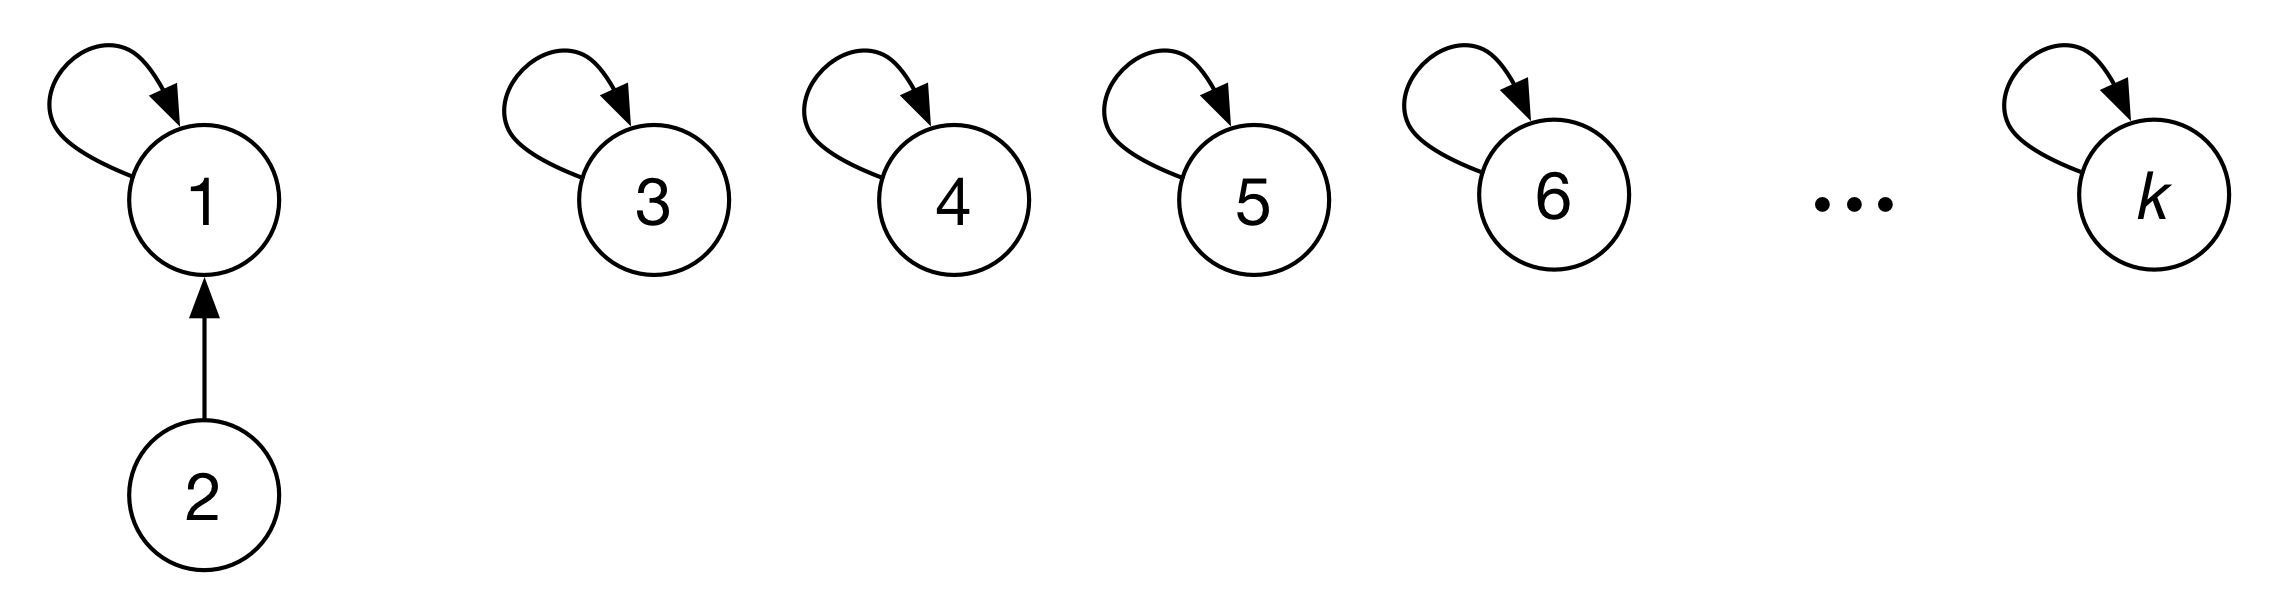
\includegraphics[scale=0.4]{images_union-find2} \par}

As another example, if we do $union(3,4)$, we get:

{\centering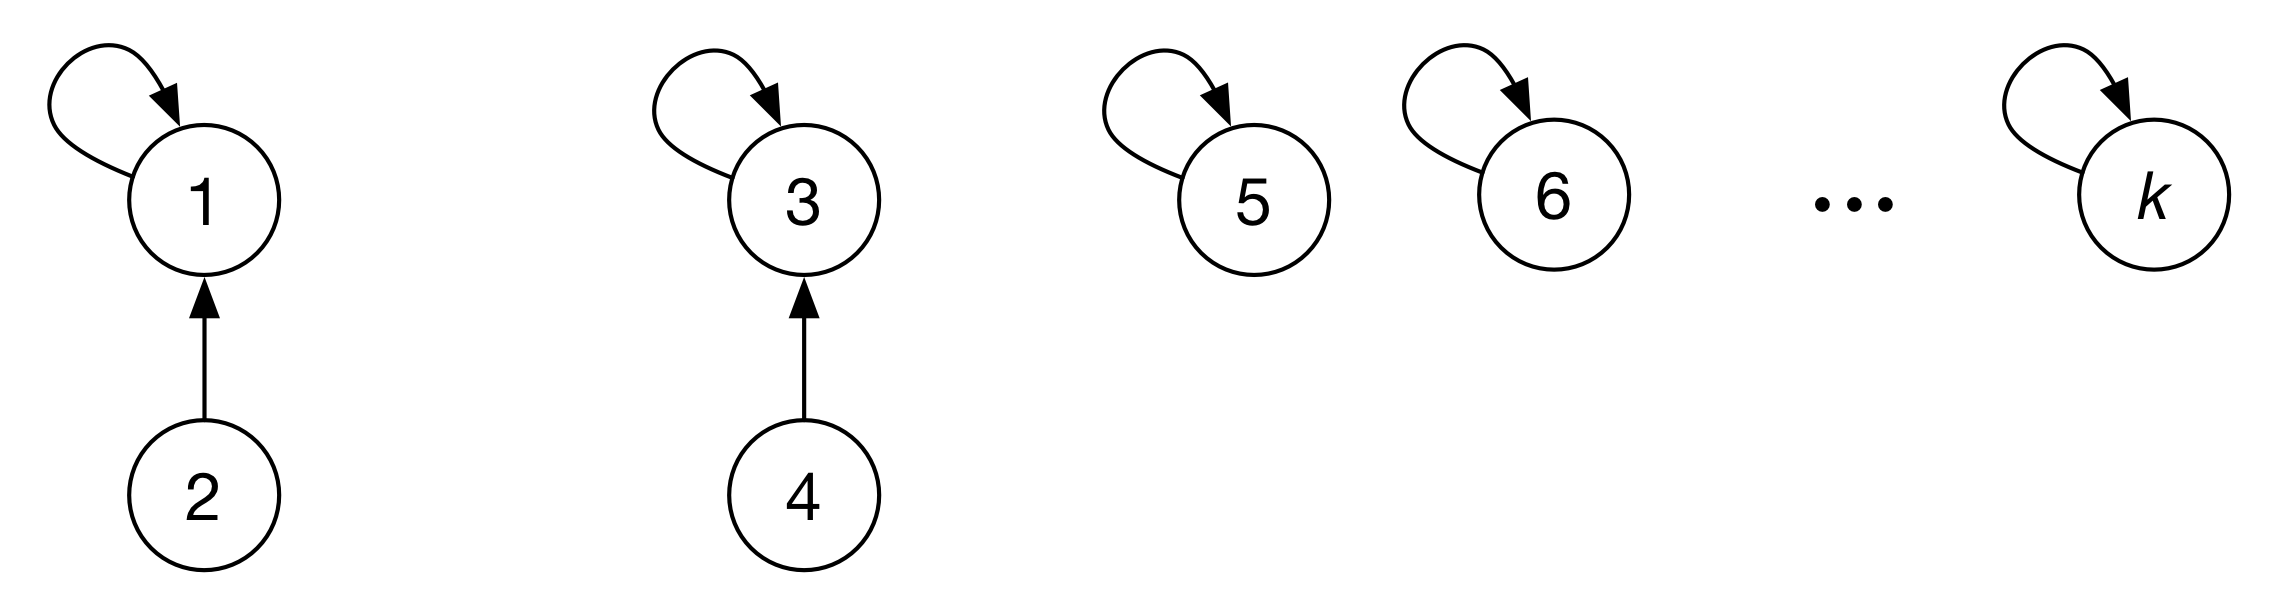
\includegraphics[scale=0.4]{images_union-find3} \par}

Thus, now nodes 1 and 2 belong to the same connected component since for either of the nodes, if we keep following the directed edges (the arrows), we end up at the same node 1 that is its own parent. Similarly, nodes 3 and 4 belong to the same connected component. In particular, this illustrates how the $find$ function works: $find(i)$ simply goes to node $i$ and keeps following the directed arrows until it hits a node that is its own parent: nodes that are their own parents are the unique representatives of each connected component. If you want, you can think of each connected component as a group where there is a leader of the group, which is the node that is its own parent, and $find(i)$ returns whoever this leader node is. Thus, at this point $find(1)=1$, $find(2)=1$, $find(3)=3$, $find(4)=3$, etc.

Importantly, what's going to cause $find$ to be slow is if we have to follow a lot of arrows. To prevent the graphs formed from in some sense becoming ``unbalanced'', the $union$ function needs to be careful with how it combines connected components.

Consider if we want to do $union(3,5)$. A bad idea would be to have node 5's parent be changed to be node 4. This makes it so that $find(5)$ would have to move along 2 edges before reaching 3. A better idea is to have node 5's parent be changed to node 3:

{\centering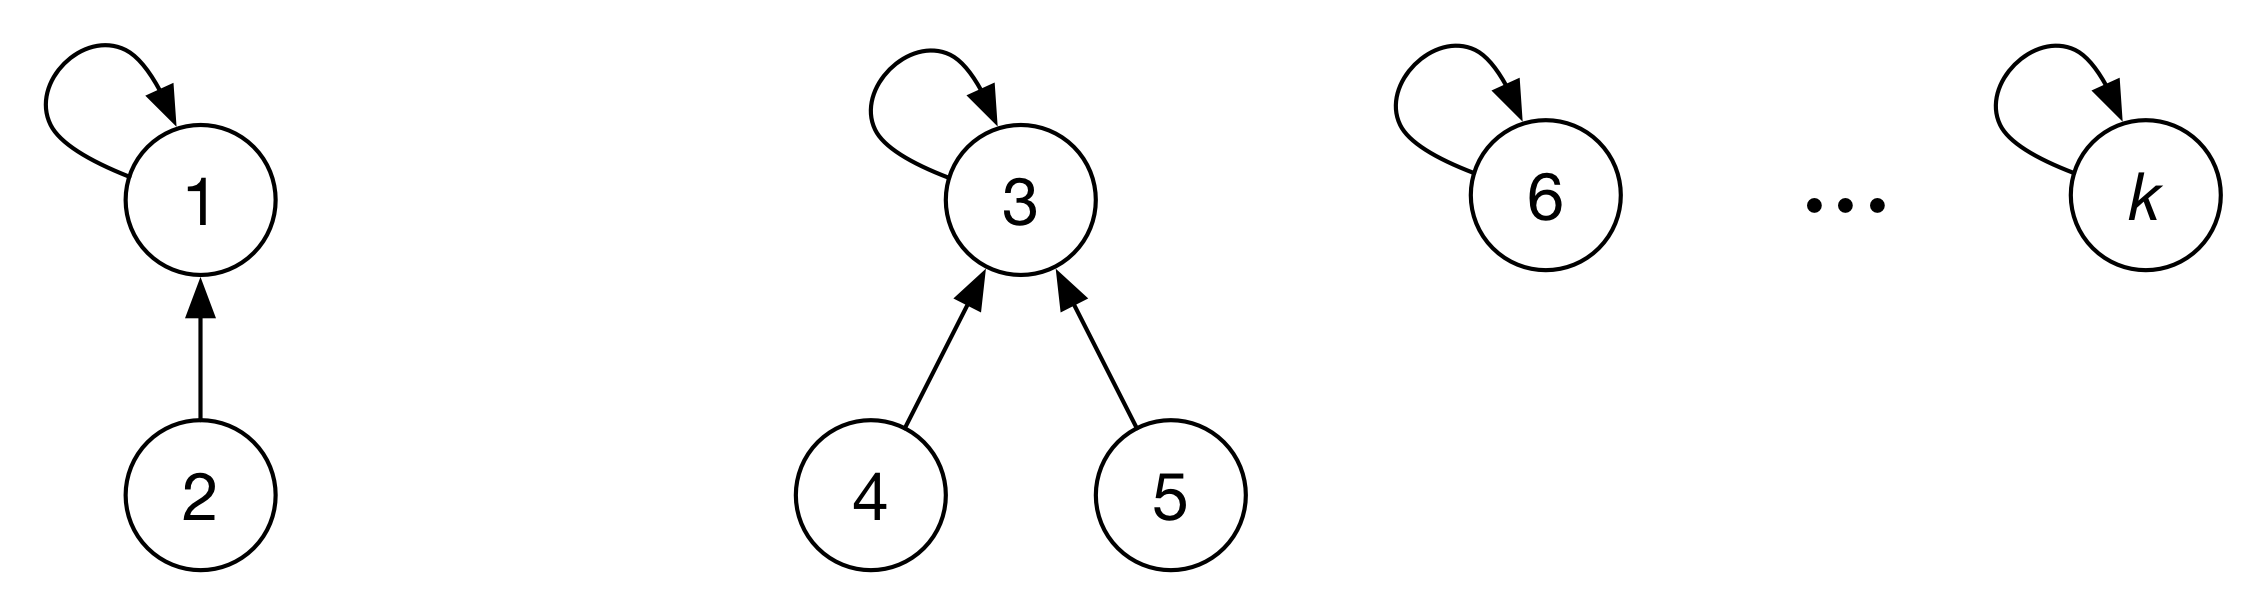
\includegraphics[scale=0.4]{images_union-find4} \par}

In particular, the basic idea is that we take the shorter tree and set its root to be the root of the taller tree.

Of course, some times the heights are the same, so we're forced to just make a taller tree. For example, $union(2,5)$ yields the following:

{\centering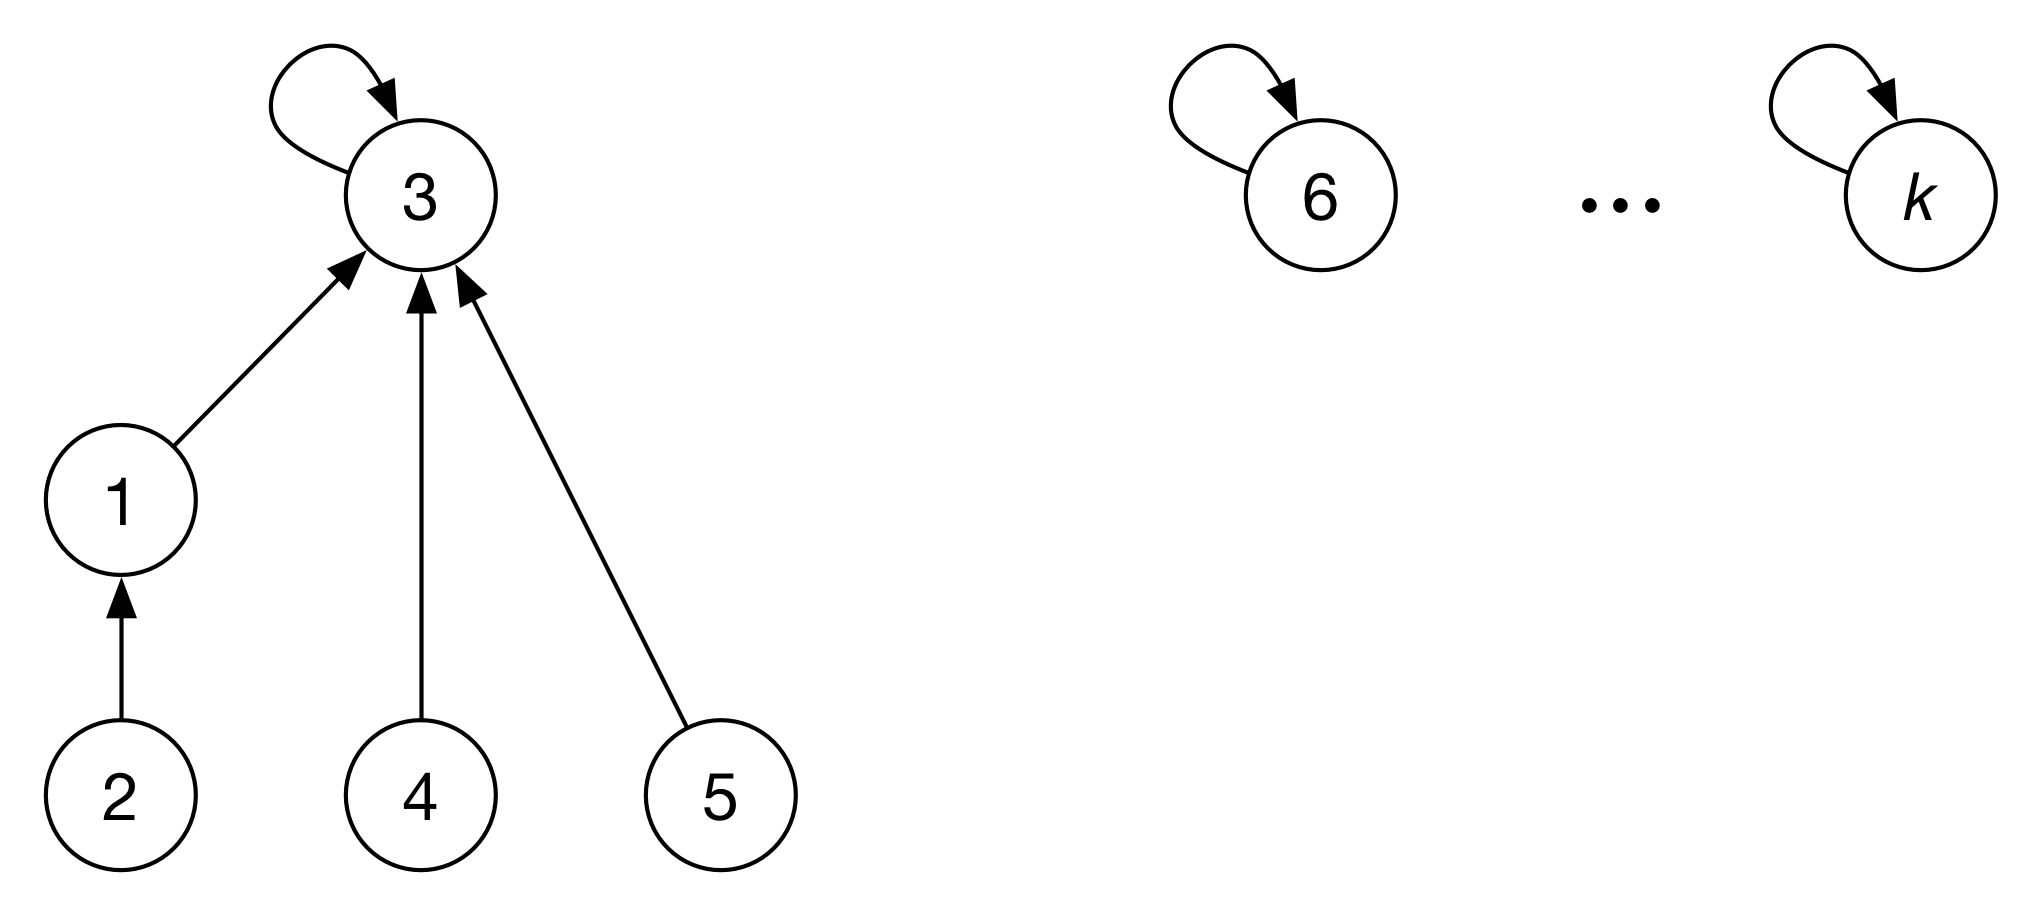
\includegraphics[scale=0.4]{images_union-find5} \par}

To help with figuring out which tree is higher, for every node, the Union-Find data structure stores a variable $rank$ that says how tall that node is. For example, below we have written out all the ranks:

{\centering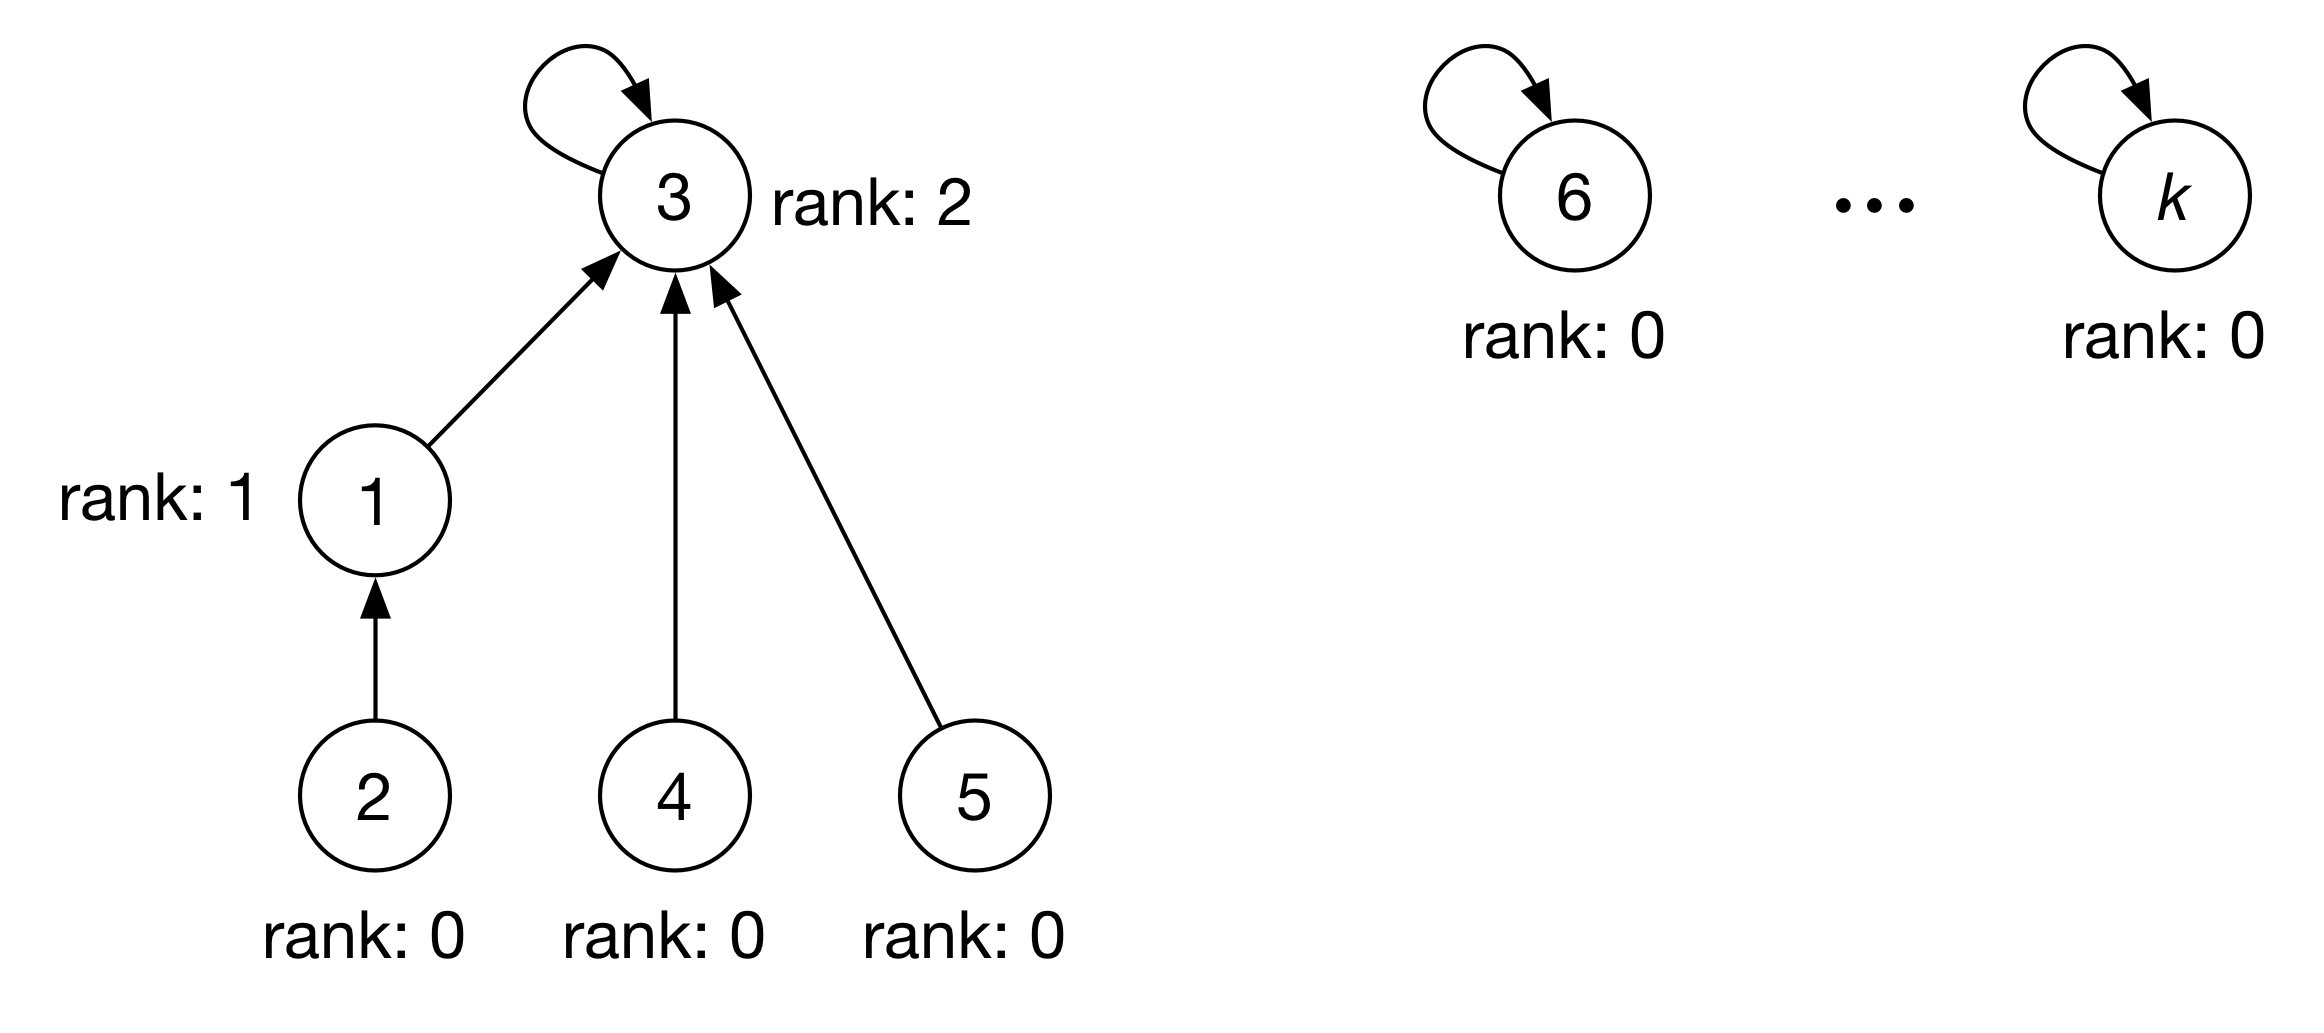
\includegraphics[scale=0.4]{images_union-find6} \par}

We are now ready to provide detail for the three operations of the Union-Find data structure.

\textbf{Initialization.}

\-\hspace{7mm} For each node $i\in \{ 1,\dots ,k\}$:

\-\hspace{12mm} Set $\pi(i)=i$. (Set the parent of node $i$ to be $i$.)

\-\hspace{12mm} Set $rank(i)=0$. (Set the height of node $i$ to be 0.)

\textbf{find$(i)$:}

\-\hspace{7mm} While $i\ne \pi (i)$: (While we have not reached the node that is its own parent:)
        
\-\hspace{12mm} Set $i=\pi(i)$. (Follow the directed edge upward.)
				
\-\hspace{7mm} Return $i$. (Return the ``leader'' of the connected component which is the node that is its own parent.)

\textbf{union$(i,j)$:}

\-\hspace{7mm} Set $r_i=find(i)$. (Find the root of the connected component of $i$.)

\-\hspace{7mm} Set $r_j=find(j)$. (Find the root of the connected component of $j$.)

\-\hspace{7mm} If $r_i=r_j$: (If the connected components are the same:)

\-\hspace{12mm} Return. (There's nothing to do since $i$ and $j$ are already in the same connected component.)

\-\hspace{7mm} Else:

\-\hspace{12mm} If $rank(r_i)>rank(r_j)$: (If the tree rooted at $r_i$ is taller than the tree rooted at $r_j$:)

\-\hspace{18mm} Set $\pi(r_j)=r_i$. (Change the parent of $r_j$ to be the root $r_i$ of the taller tree.)

\-\hspace{12mm} Else:

\-\hspace{18mm} Set $\pi(r_i)=r_j$. (Change the parent of $r_i$ to be the root $r_j$ of the same height or taller tree.

\-\hspace{18mm} If $rank(r_i)=rank(r_j)$: (If they were actually the same height:)

\-\hspace{24mm} Set $rank(r_j)=rank(r_j)+1$. (Change the height of the now taller root node to be 1 taller.)

Running time for the three pieces: It should be clear why initialization takes time $\mathcal{O}(k)$ i.e., linear in the number of nodes. A more careful argument is needed to justify why the rank of any node is at most $\log_2 k$, which would immediately imply that each $fin$d call takes $\mathcal{O}(\log k)$ time (since the rank is how high a node in a tree is and the running time of $find$ just scales with the maximum height of a tree, which is the maximum rank). Meanwhile, each call to $union$ involves calling $find$ twice followed by a series of operations that takes time $\mathcal{O}(1)$, so the overall running time for each union call is the same as that of find, namely $\mathcal{O}(\log k)$.

The question that remains is why the rank of any node is at most $\log_2 k$. To answer this, we make a series of observations that build on each other:

\begin{itemize}
\item As we move upward along any directed edge, the rank strictly increases. In other words, $rank(i)<rank(\pi(i))$.

\item The only time we ever increment a rank of a root node is when we just did a union of two trees that have the same height (for which for exactly one of the original root nodes, we increase its rank by 1). This means that the very first time we do union (for example, when we start from everything disconnected and we do our very first $union$), the smallest possible two trees we are merging each has size 1, and the resulting tree ends up having rank 1 and 2 nodes. Thus, we need at least 2 of these rank 1 trees with at least 2 nodes each to form a bigger tree with rank 2, at which point we at least have 4 nodes. This pattern continues: The (sub)tree rooted at a node with rank $\ell$ must have at least $2^{\ell}$ nodes in it.

\item How large could the largest rank possibly be? Well, since a rank $\ell$ node has at least $2^{\ell}$ nodes in it, consider when $\ell =\log _{2}k$, which means that this tree as at least $k$ nodes in it, but this is indeed the total number of nodes! Thus, we cannot have a higher rank than $\ell =\log _{2}k$; otherwise, we would need more than $k$ nodes.
\end{itemize}

This completes our analysis of the Union-Find data structure.

\textbf{Path compression.} We end by stating a remarkable result. It turns out that there's a small modification to find that cuts down the running time for each call to find to take \textit{average} running time $\mathcal{O}(\log_2^{*} k)$ instead of $\mathcal{O}(\log k)$, where $\log_2^{*}$ (pronounced log star) is the iterated logarithm, i.e., how many times you iteratively apply log base 2 until you get a number at most 1. Note that $\log_2^{*}$ grows extremely slowly: $\log _2^*(2^{65536}) = 5$, and $2^{65536}$ is many orders of magnitude larger than the number of atoms in the observable universe ($\approx 10^{80}$). As such, for practical purposes, $\mathcal{O}(\log_2^{*} k)$ might as well be constant time.

The trick is that when we call $find(i)$, for every node we encounter as we work our way to the ``leader''/root node, we change all the parents of nodes we encounter to directly point to the ``leader''/root node. This makes it so that $rank$ no longer corresponds to tree height, but it turns out to not affect correctness. Now the tree height gets compressed quite substantially. This modification is called “path compression".

The only change is in the $find$ procedure:

\textbf{find($i$):}

    If $i\ne \pi (i)$: (If node $i$ is not a ``leader''/root node:)

        Set $\pi(i)=find(\pi(i))$. (Change the parent of $i$ to be the ``leader''/root node.)

    Return $\pi(i)$. (Return the ``leader''/root node.)

We can readily unravel the recursion: if $i$ is a ``leader''/root node, we skip the if statement and just return the node itself since it is its own parent. Otherwise, we recursively work our way up the directed tree changing parents of the nodes we encounter to all point to the ``leader''/root node.

The running time analysis here requires looking at an ``amortized'' or averaged case over a sequence of $find$ calls, which we will omit details for.

The bottom line is that the average case running time of Kruskal's algorithm with this path compression modification makes it so that the $find$ and $union$ calls (again each $union$ call does two $find$ calls, which dominates its running time) each takes average time $\mathcal{O}(\log _2^* k)$, yielding an overall average running time of

{\centering$\underbrace{\mathcal{O}(1)+\mathcal{O}(k)}_{\text {initialization}} +\underbrace{\mathcal{O}(k^{2}\log k)}_{\text {sorting}} +\underbrace{{k \choose 2}\big (\mathcal{O}(\log _2^* k)+\mathcal{O}(1)+\mathcal{O}(\log _2^* k)\big )}_{\text {adding edges}} =\mathcal{O}(k^{2}\log k + k^2\log _2^* k).$ \par}
 
The sorting operation still dominates the running time, but if the edge weights can be converted to limited precision unsigned integers without sacrificing accuracy (i.e., by converting floating point to integers, so long as the different edges still correspond to different integers and no two edge weights get quantized to be the same integer when they were different weights before), then a linear-time radix sort can be used, bringing the average running time of this modified Kruskal's algorithm to

{\centering$\mathcal{O}(p k^{2} + k^2\log _2^* k),$ \par}
 
where $p$ is an integer precision parameter, which you can think of as scaling with the maximum number of bits needed to store the integers used to represent the edge weights. With this modification, the overall Chow-Liu algorithm with path compression and radix sort has running time

{\centering$\mathcal{O}(k^{2}|\mathcal{X}|^{2}n + p k^{2} + k^2\log _2^* k),$ \par}
 
cut down from the original Chow-Liu running time of

{\centering$\mathcal{O}(k^{2}|\mathcal{X}|^{2}n+k^{2}\log k),$ \par}
 
where $k$ is the number of random variables in the graph, $|\mathcal{X}|$ is the (maximum) alphabet size of any of the random variables, and $n$ is the number of training data points, Again, we need the additional assumption on the precision of the edge weights being sufficiently limited to enable radix sort.



\end{document}
